\documentclass[pt=100]{article}
\title{\textbf{\textit{\emph{M}aking \emph{G}raphs}}}
\author{\textbf{Sofiullah Iqbal Kiron}}
\date{\textbf{\today}}

\usepackage
{
	graphicx,
	tkz-graph,
	pgfplots,
	color,
	listings,
	mathtools
}

\lstset
{
 language=C++,
 backgroundcolor=\color{black!10!green!10},
 basicstyle=\footnotesize\ttfamily,
 keywordstyle=\color{blue},
 commentstyle=\color{green!80},
 showstringspaces=false,
 stringstyle=\color{red},
 captionpos=b
}

\begin{document}
\maketitle

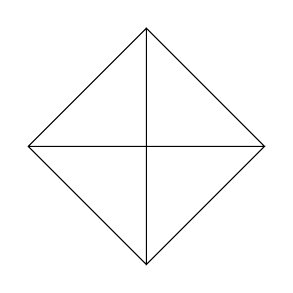
\begin{tikzpicture}

%Now I'm gonna drowing here a square by co-ordinate system.
\draw(-1.5, 0)--(1.5, 0)--(0, -1.5)--(0, 1.5)--(1.5, 0)--(0, 1.5)--(-1.5, 0)--(0, -1.5);
\draw;

\end{tikzpicture}

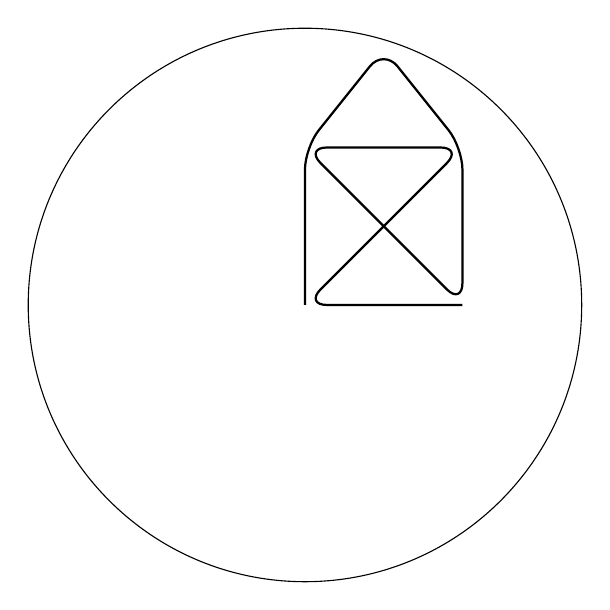
\begin{tikzpicture}
 \draw[thick, rounded corners=8pt]
(0,0) -- (0,2)-- (1,3.25) -- (2,2) -- (2,0) -- (0,2) -- (2,2) -- (0,0) -- (2,0);
 \draw(0, 0) circle [radius = 100 pt];
\end{tikzpicture}

\begin{tikzpicture}
 
\end{tikzpicture}

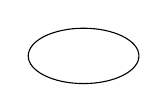
\begin{tikzpicture}
 \draw(10, 0) ellipse[x radius = 20 pt, y radius = 10 pt];
\end{tikzpicture}

\begin{tikzpicture}

 \draw (-1.5,0) -> (1.5,0);
 \draw (0,-1.5) -> (0,1.5);

\end{tikzpicture}

We are working on blah:\\One unit is 1 cm initially.
\begin{tikzpicture}

 \draw (-2.5,0) -- (2.5,0);
 \draw (0,-2.5) -- (0,2.5);

\end{tikzpicture}

\tikz
{
\draw(0, 0) -- (1.5, 2);
\draw(0, 0) -- (1.5, 0) -- (1.5, 2) %If there is onec more draw command, so there is no need to add semicolon.
}

\tikz
{

 \filldraw[blue] (0, 0)circle [radius = 4pt];
 \filldraw[blue] (1, 1)circle [radius = 4pt];
 \filldraw[blue] (2, 1)circle [radius = 4pt];
 \filldraw[blue] (1, 2)circle [radius = 4pt];
 \draw (0, 0) .. controls(1, 2) .. (2, 1);
 
}

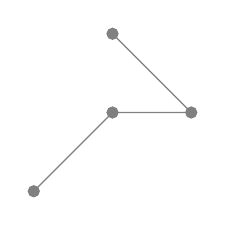
\begin{tikzpicture}

 \filldraw[gray]
 (0, 0)circle [radius = 2pt]--
 (1, 1)circle [radius = 2pt]--
 (2, 1)circle [radius = 2pt]--
 (1, 2)circle [radius = 2pt];
 
\end{tikzpicture}

\tikz
{

 \draw(-1.5, 0)--(1.5, 0);
 \draw(0, -1.5)--(0, 1.5);
 \draw(-1, 0)..controls(0, 1)..(1, 0);
 \draw[green](0, 0) circle[radius=15 pt];

}

\tikz
{

 \draw(-1.5, 0)--(1.5, 0);
 \draw(0, -1.5)--(0, 1.5);
 \filldraw[green](0, 0) circle[radius=1 cm]; %cm is so long in LaTeX compiler.

}

\tikz
{

 \draw(-1.5, 0)--(1.5, 0);
 \draw(0, -1.5)--(0, 1.5);
 \filldraw[gray](0, 0.5)rectangle(0.5, 0);

}

\tikz
{

 \draw[blue, step=0.3 cm, rotate=0](-2, -2)grid(2, 2);
 \filldraw[green!53](0, 0) circle[radius=1 cm];
 \draw(-1.5, 0)--(1.5, 0);
 \draw(0, -1.5)--(0, 1.5);
 
}

\tikz
{

 \draw(-1.5, 0)--(1.5, 0);
 \draw(0, -1.5)--(0, 1.5);
 \filldraw[green](0, 1)--(1, 0)--(0, 0)--(0, 1);

}

\tikzset
{
	mygrid/.style={color=blue, thin}
}

\tikz
{

	\draw[step=1 cm, yellow, very thick](-5, -5)grid(5, 5);
	\filldraw[mygrid](0, 2) circle[radius=1 cm];
}

\tikz
{
	\draw(0, 2)node[shape=circle, color=green, radius=4 cm, draw]{Sofiul};
	\draw(2, 0)node[style=rectangle, color=green, draw]{Kiron};
	\draw(0, 0)node[style=rectangle, color=gray, draw]{Sofi};
}

\tikzset
{
	setu/.style={circle, blue!79, draw, fill=yellow!50}
}

\tikz
{
	\path
	 (0, 0)node[setu]{A}
	 (0, -1)node[setu]{B}
	 (-1, 0)node[setu]{C}
	 (0, 1)node[setu]{D}
	 (1, 0)node[setu]{E};
}

\tikz
{ %If do not add "at" syntax, all the names placed in 1 point.

	 \node[fill=yellow!56, rectangle](A) at (0, 0){A};
	 \node(B) at (0, -1)[setu]{B};
	 \node(C) at (-1, 0)[setu]{C};
	 \node(D) at (0, 1)[setu]{D};
	 \node(E) at (1, 0)[setu]{E};
	 \draw[red, ->](A) -- (C);
	 \draw[red, ->](C) ..controls(-1, 0.3) and (-1, 0.9).. (D);
	 \draw[red, ->](D) ..controls (2.1, 0.7) and (2.1, -0.7).. (B);
	 \draw[red, ->](B) -- (E);
}

\tikz
{ %Here, I will add labels on node.

	 \node[fill=yellow!56, rectangle](A) at (0, 0){A};
	 \node(B) at (0, -1)[setu]{B};
	 \node(C) at (-1, 0)[setu]{C};
	 \node(D) at (0, 1)[setu]{D};
	 \node(E) at (1, 0)[setu]{E};
	 \draw[red, ->](A) -- (C);
	 \draw[red, ->](C) ..controls(-1, 0.3) and (-1, 0.9).. (D);
	 \draw[red, ->](D) ..controls (2.1, 0.7) and (2.1, -0.7).. (B);
}

\tikzset
{
	Vertex/.style={draw, circle, blue, fill=green!60!yellow}
}

\tikz
{
	\node(V1) at (-3, 2)[Vertex] {V1};
	\node(V2) at (0, 0)[Vertex] {V2};
	\node(V3) at (4, 0)[Vertex] {V3};
	\node(V4) at (7, 2)[Vertex] {V4};
	\node(V5) at (10, 0)[Vertex] {V5};
	\node(V6) at (7, -2)[Vertex] {V6};
	\node(V7) at (-3, -2)[Vertex] {V7};
	\draw [blue!10!green, ->, thick] (V1) -- (V2);
	\draw [blue!10!green, ->, thick] (V2) -- (V3);
	\draw [blue!10!green, ->, thick] (V3) -- (V4);
	\draw [blue!10!green, ->, thick] (V4) -- (V5);
	\draw [blue!10!green, ->, thick] (V5) -- (V6);
	\draw (V6) -- (V3);
	\draw (V2) -- (V7) -- (V1);
	
}

\tikz
{

	\draw (0, 0)--(-1.9, 1)..controls(-2.2, 2) and(-3.9, 2.2)..(-4.1, 0.2);
	\draw (0, 0)--(-2, -0.5)..controls(-3.9, -3.8) and(-7.2, -3.3)..(-8.6, -1.9);
	\draw (-8.6, -1.9)..controls(-10.8, -0.4)..(-13, 0.8);
	\draw (-4.1, 0.2)..controls(-6.8, 0.3)..(-8.5, -0.4)--(-13, 0.8);
	\draw (-3.9, -2.4)--(-4, -3.8)--(-4.35, -4.2);

}

\tikzset
{
	place/.style={draw, blue, circle, radius=2 pt, fill=green!49}
}

\tikz
{

	\node(One) at (0, 0)[place]{M};
	\node[red, above] at (One.north){$s\le3$};
}

\tikz
{
	\node {root}
	 child {node {left}}
	 child {node {middle}}
	 child {node {right}
	  child {node {second}}}
}

\tikz
{
	\node
	 {1}
	  child {node {1.1} child {node {1.1.1}} child {node {1.1.2}} child {node {1.1.3}} }
	  child {node {1.2}}
	  child {node {1.3}}
	    
}

\section{Binary Tree Illustration}
Here is the illustration of some \textcolor{blue}{Binary Trees}. Trees are a common way of visualizing hierarchical data structures. A computer scientist's trees grow downward while a mathematician's tree will grow upward.\hfill
Two binary tree will said to be similar if they both have same structure and said to be copy if they have same structure and same content at corresponding node.\hfill

\begin{center}
	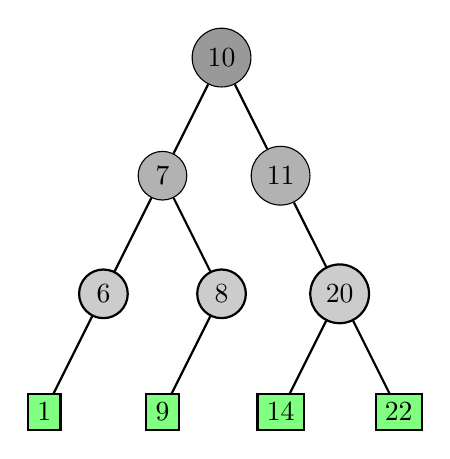
\begin{tikzpicture}[edge from parent/.style={draw, thick}]
		\node[fill=gray!80, circle, draw](10) {10} [grow=down]
	 		child {node[fill=gray!60, circle, draw](7) {7} %edge from parent[->] %Level 2
	 			child {node[fill=gray!40, circle, draw](6) {6}
	 				child {node[fill=green!50, rectangle, draw](1) {1}}
	 				child[missing]}
	 			child {node[fill=gray!40, circle, draw](8) {8}
	 				child {node[fill=green!50, rectangle, draw](9) {9}}
	 				child[missing]}}
	 		child {node[fill=gray!60, circle, draw](11) {11} %edge from parent[->] %Level 2
	 		    child[missing]
	 			child {node[fill=gray!40, circle, draw](20) {20}
	 				child {node[fill=green!50, rectangle, draw](14) {14}}
	 				child {node[fill=green!50, rectangle, draw](22) {22}}}};
	 	%\node[violet, above] at (10.north){nlr};
	 	%\node[violet, above] at (7.north){nlr};
	\end{tikzpicture}
\end{center}
Internal nodes are represented by circle and external nodes or leafs are represented by rectangle / square.
\subsection{Kinds of binary tree}
\begin{enumerate}
    %Item 1.
	\item \textbf{Full binary tree:} In every node for a tree that has either $0$ or $2$ child nor $1$.\linebreak
	\tikz
	{
		\node[draw, circle] {A} [grow=down]
			child {node[draw, circle] {B}}
			child {node[draw, circle] {C}
				child {node[draw, rectangle] {D}}
				child {node[draw, rectangle] {E}}}
	}\linebreak
	\item \textbf{Complete binary tree:} All the leafs are in same level.\linebreak
	\tikz
	{
		\node[draw, circle] {A} [grow=down]
			child {node[draw, rectangle] {B}}
			child {node[draw, rectangle] {C}}
	}\linebreak
	\item \textbf{Perfect binary tree:}
\end{enumerate}

\subsection{Binary tree traverse}
There are \textcolor{red}{three} $(3)$ standard algorithm to traverse the binary tree. Those are:-\hfill
\begin{enumerate}
	\item \textbf{Preorder} (\textit{nlr})
	\item \textbf{Inorder} (\textit{lnr})
 	\item \textbf{Postorder} (\textit{lrn})
\end{enumerate}
Okay, now this is the time for describing this three\dots\hfill

\begin{enumerate}
	\item \textbf{Preorder}
		\begin{enumerate}
			\item Process the root.
			\item Process the left subtree.
			\item Process the right subtree.\hfill
		\end{enumerate}
		So we can easily say that, the form is \textit{nlr}. Let's traverse previous binary tree by this \textit{nlr} form.\hfill
\begin{center}
	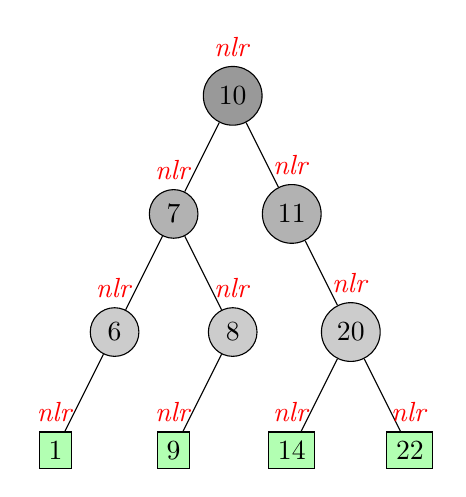
\begin{tikzpicture}
		\node[fill=gray!80, circle, draw](10) {10} [grow=down]
	 		child {node[fill=gray!60, circle, draw](7) {7}
	 			child {node[fill=gray!40, circle, draw](6) {6}
	 				child {node[fill=green!30, rectangle, draw](1) {1}}
	 				child[missing]}
	 			child {node[fill=gray!40, circle, draw](8) {8}
	 				child {node[fill=green!30, rectangle, draw](9) {9}}
	 				child[missing]}}
	 		child {node[fill=gray!60, circle, draw](11) {11}
	 		    child[missing]
	 			child {node[fill=gray!40, circle, draw](20) {20}
	 				child {node[fill=green!30, rectangle, draw](14) {14}}
	 				child {node[fill=green!30, rectangle, draw](22) {22}}}};
	 	\node[red, above] at (10.north){\textit{nlr}};
	 	\node[red, above] at (7.north){\textit{nlr}};
	 	\node[red, above] at (6.north){\textit{nlr}};
	 	\node[red, above] at (1.north){\textit{nlr}};
	 	\node[red, above] at (8.north){\textit{nlr}};
	 	\node[red, above] at (9.north){\textit{nlr}};
	 	\node[red, above] at (11.north){\textit{nlr}};
	 	\node[red, above] at (20.north){\textit{nlr}};
	 	\node[red, above] at (14.north){\textit{nlr}};
	 	\node[red, above] at (22.north){\textit{nlr}};
	\end{tikzpicture}
\end{center}
Now we obtain that list by \textbf{Preorder Traverse:} $[10, 7, 6, 1, 8, 9, 11, 20, 14, 22]$.\hfill
If we look out deeply in the traversed list, we gather that, in Preorder traverse:-\hfill
\begin{itemize}
	\item[$\rightarrow$] First element is head node.
	\item[$\rightarrow$] and rightmost element are placed in last, that's mean, last element is the rightmost leaf of considered binary tree.
\end{itemize}

\item \textbf{Inorder:}
	\begin{enumerate}
		\item Process the left subtree.
		\item Process the root.
		\item Process the right subtree.
	\end{enumerate}
	The form for the \textbf{Inorder} traversal is \textit{lnr}.\hfill
\begin{center}
	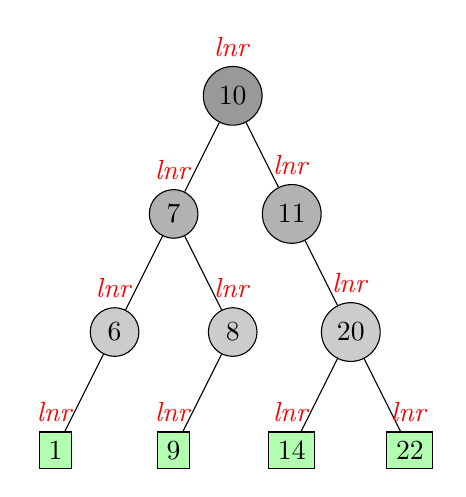
\begin{tikzpicture}
		\node[fill=gray!80, circle, draw](10) {10} [grow=down]
	 		child {node[fill=gray!60, circle, draw](7) {7}
	 			child {node[fill=gray!40, circle, draw](6) {6}
	 				child {node[fill=green!30, rectangle, draw](1) {1}}
	 				child[missing]}
	 			child {node[fill=gray!40, circle, draw](8) {8}
	 				child {node[fill=green!30, rectangle, draw](9) {9}}
	 				child[missing]}}
	 		child {node[fill=gray!60, circle, draw](11) {11}
	 		    child[missing]
	 			child {node[fill=gray!40, circle, draw](20) {20}
	 				child {node[fill=green!30, rectangle, draw](14) {14}}
	 				child {node[fill=green!30, rectangle, draw](22) {22}}}};
	 	\node[red, above] at (10.north){\textit{lnr}};
	 	\node[red, above] at (7.north){\textit{lnr}};
	 	\node[red, above] at (6.north){\textit{lnr}};
	 	\node[red, above] at (1.north){\textit{lnr}};
	 	\node[red, above] at (8.north){\textit{lnr}};
	 	\node[red, above] at (9.north){\textit{lnr}};
	 	\node[red, above] at (11.north){\textit{lnr}};
	 	\node[red, above] at (20.north){\textit{lnr}};
	 	\node[red, above] at (14.north){\textit{lnr}};
	 	\node[red, above] at (22.north){\textit{lnr}};
	\end{tikzpicture}
\end{center}
When we traverse the tree in \textit{lnr} form, we obtain that list: $[1, 6, 7, 9, 8, 10, 11, 14, 20, 22]$.\hfill
If you look at the core of the list, then you simply see that:-\hfill
\begin{itemize}
	\item[$\rightarrow$] First element in the list is leftmost node of that tree.
	\item[$\rightarrow$] Last element in the list is rightmost node of that tree.
\end{itemize}

\item \textbf{Postorder:} traversal form is \textit{lrn}.\hfill
	\begin{enumerate}
		\item Process the left subtree.
		\item Process the right subtree.
		\item at last, process the node.
	\end{enumerate}

\begin{center}
	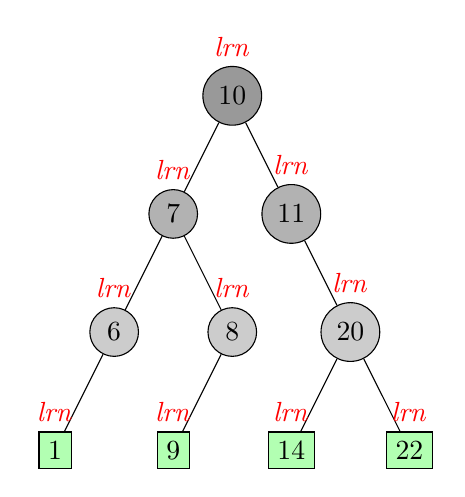
\begin{tikzpicture}
		\node[fill=gray!80, circle, draw](10) {10} [grow=down]
	 		child {node[fill=gray!60, circle, draw](7) {7}
	 			child {node[fill=gray!40, circle, draw](6) {6}
	 				child {node[fill=green!30, rectangle, draw](1) {1}}
	 				child[missing]}
	 			child {node[fill=gray!40, circle, draw](8) {8}
	 				child {node[fill=green!30, rectangle, draw](9) {9}}
	 				child[missing]}}
	 		child {node[fill=gray!60, circle, draw](11) {11}
	 		    child[missing]
	 			child {node[fill=gray!40, circle, draw](20) {20}
	 				child {node[fill=green!30, rectangle, draw](14) {14}}
	 				child {node[fill=green!30, rectangle, draw](22) {22}}}};
	 	\node[red, above] at (10.north){\textit{lrn}};
	 	\node[red, above] at (7.north){\textit{lrn}};
	 	\node[red, above] at (6.north){\textit{lrn}};
	 	\node[red, above] at (1.north){\textit{lrn}};
	 	\node[red, above] at (8.north){\textit{lrn}};
	 	\node[red, above] at (9.north){\textit{lrn}};
	 	\node[red, above] at (11.north){\textit{lrn}};
	 	\node[red, above] at (20.north){\textit{lrn}};
	 	\node[red, above] at (14.north){\textit{lrn}};
	 	\node[red, above] at (22.north){\textit{lrn}};
	\end{tikzpicture}
\end{center}
By traversing in postorder algo., we obtain: $[1, 6, 9, 8, 7, 14, 22, 20, 11, 10]$.\\\\
\hspace{1 cm}Now, look at the list deeply:-\hfill
\begin{itemize}
	\item[$\rightarrow$] First element of the list is leftmost leaf of the considered binary tree.
	\item[$\rightarrow$] Last element of the list is head-node of the considered binary tree.
\end{itemize}
	
\end{enumerate}

\subsection{Binary tree implementation}
A binary tree contains $3$ parts at a node:-
\begin{enumerate}
	\item Data
	\item Pointer to the left subtree.
	\item Pointer to the right subtree.
\end{enumerate}

As we assume:-
\begin{center}
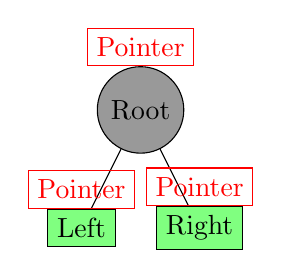
\begin{tikzpicture}
{
	\node[fill=gray!80, circle, draw] (Root) {Root}
		child {node[fill=green!50, rectangle, draw] (Left) {Left}}
		child {node[fill=green!50, rectangle, draw] (Right) {Right}};
	\node[red, above, draw, rectangle] at (Root.north){Pointer};
	\node[red, above, draw, rectangle] at (Left.north){Pointer};
	\node[red, above, draw, rectangle] at (Right.north){Pointer};
}
\end{tikzpicture}
\end{center}

We need a struct for implement this. For the illustration purpose in C++ language:-\hfill
\begin{lstlisting}[caption = struct for node, numbers = left]
	struct node
	{
		int data;
		node *left, *right;
	};
\end{lstlisting}

Then we need a function for make node, namely make\_node.\hfill
\begin{lstlisting}[caption = Function for make a new node, numbers = left]
node *make_node(int value)
{
    node *new_node = new node;
    new_node->data = value;
    new_node->left = NULL;
    new_node->right = NULL;
}
\end{lstlisting}

Three type of Traverse code:-\hfill
\begin{enumerate}

	\item If we wanna traverse the tree in Preorder form, then use the following code:-\hfill
	\begin{lstlisting}[caption = Void function for preorder traverse, numbers = left]
void preorder(node *root)
{
    if (root != NULL)
    {
        cout << root->data;
        preorder(root->left);
        preorder(root->right);
    }
}
	\end{lstlisting}
	
	\item Else if we traverse the tree in Inoreder form by this code:-\hfill
	\begin{lstlisting}[caption = Void function for preorder traverse, numbers = left]
void inorder(node *root)
{
    if (root != NULL)
    {
        inorder(root->left);
        cout << root->data;
        inorder(root->right);
    }
}
	\end{lstlisting}
	
	\item Or traverse Postorder form by this void code:-\hfill
	\begin{lstlisting}[caption = Void function for preorder traverse, numbers = left]
void postorder(node *root)
{
    if (root != NULL)
    {
        postorder(root->left);
        postorder(root->right);
        cout << root->data;
    }
}
		\end{lstlisting}
	
\end{enumerate}

\subsection{Properties and application}
There is an equation such as:- $E = (a-b) / (c * d) + e$. This equation can be represented by a binary tree as:\\
\begin{center}
\tikz
[
	level distance=15mm,
	level 1/.style={sibling distance=20mm},
	level 2/.style={sibling distance=12mm},
	level 3/.style={sibling distance=12mm}
]
{
	\node[draw, circle] {/}
		child{node[draw, circle] {-}
			child {node[draw, rectangle] {a}}
			child {node[draw, rectangle] {b}}}
		child{node[draw, circle] {+}
			child {node[draw, circle] {*}
				child {node[draw, rectangle] {c}}
				child {node[draw, rectangle] {d}}}
			child {node[draw, rectangle] {e}}}
}
\end{center}

When we labeling a binary tree in level-order process, then we gather, if parent is $k$ then:
\begin{itemize}
	\item Left child is $2k$.
	\item Right child is $2k+1$, so we can say, child of $k$ is $\{2k,\hspace{0.5mm}2k+1\}$.
	\item Parent of $k$ is $\left\lfloor\frac{k}{2}\right\rfloor$.
	\item If number of nodes is $n$ then depth, $d_n = \left\lfloor\log_2n+1\right\rfloor$.
	\item If height of tree is $h$ then total number of nodes: $n(Tn) = 2^h-1$ where $Tn$ is Total node.
\end{itemize}

\end{document}
